\setlinespacing{1.1}


\chapter{Introduction and Background} \label{sec:introduction}

\section{Title}

\begin{comment}
\subsection{Subsection header 1}
fdsdfsdfds
\subsection{Subsection header 2}
fdsdfsdfds
\subsection{Subsection header 3}
fdsdfsdfds
\end{comment}

SECURE WEB-BASED EXAM PAPER GENERATION SYSTEM

\section{Background}

\begin{comment}
\subsection{Subsection header 1}
fdsdfsdfds
\subsection{Subsection header 2}
fdsdfsdfds
\subsection{Subsection header 3}
fdsdfsdfds
\end{comment}

With every new college year and semester, lecturers are faced with the prospect of composing examination papers for the next coming months. Since this can prove to be a very tedious and physically demanding task. More over, it can also be very challenging due to the time consumption and nature of the process for the examiner. The traditional method of composing papers can be automated. Therefore, there exists an opportunity to provide a service to simplify the process. \\
The use of a Web-based examination paper generation system which makes use of a relational database and database tables to cross-reference the newly created table of randomised questions with the tables from the previous years or semester. Resulting to a non-repeating question sheet.
% in a random manor Within the tables are the records of questions which have been make use of the browser as the interface 

\section{Main Research Question(s)}

\begin{enumerate}
\begin{comment}
	\item{\bfseries Will this benefit the examiners?} \\ 
	Year on year. Examiners have a good bit to say regarding the time which it takes to compose their exams. With that being said. There is definitely a requirement for such a system.
\end{comment}
	
	\item{\bfseries What will the end user experience be like, or will they prefer the old fashion method to what they are used to?} \\
	Not everyone can adapt to change as well as others. This is why getting used to a new system could take some time. Some folk may even get frustrated to the point where they find the new interface impossible to use. This is 	not the intension. The project is meant to make the process more streamlined and user friendly. This is why a great deal will be taken in the design of the user interface to make the experience a pleasurable one.
	
	\item{\bfseries Could the presence of an automated generation of questions system improve the accuracy of questions over a manual generation?} \\
	There are many factors which can affect a human beings output when given a task. These factors could range from fatigue. Being distracted by a colleague. Or not having the focus needed to complete the task at hand. This is 	where machines have the advantage over us. Humans suffer from what is called, "Human error." Whereas a machine can produce the same output with precision and repetition. This is why an automated system would work in college environment.
\end{enumerate}

\begin{comment}
\section{section header 2}

\subsection{Subsection header 1}

Figure \ref{Figure: Map of the Greater Dublin Area} shows a spatial map of the GDA.

\begin{figure}[htbp]
\center 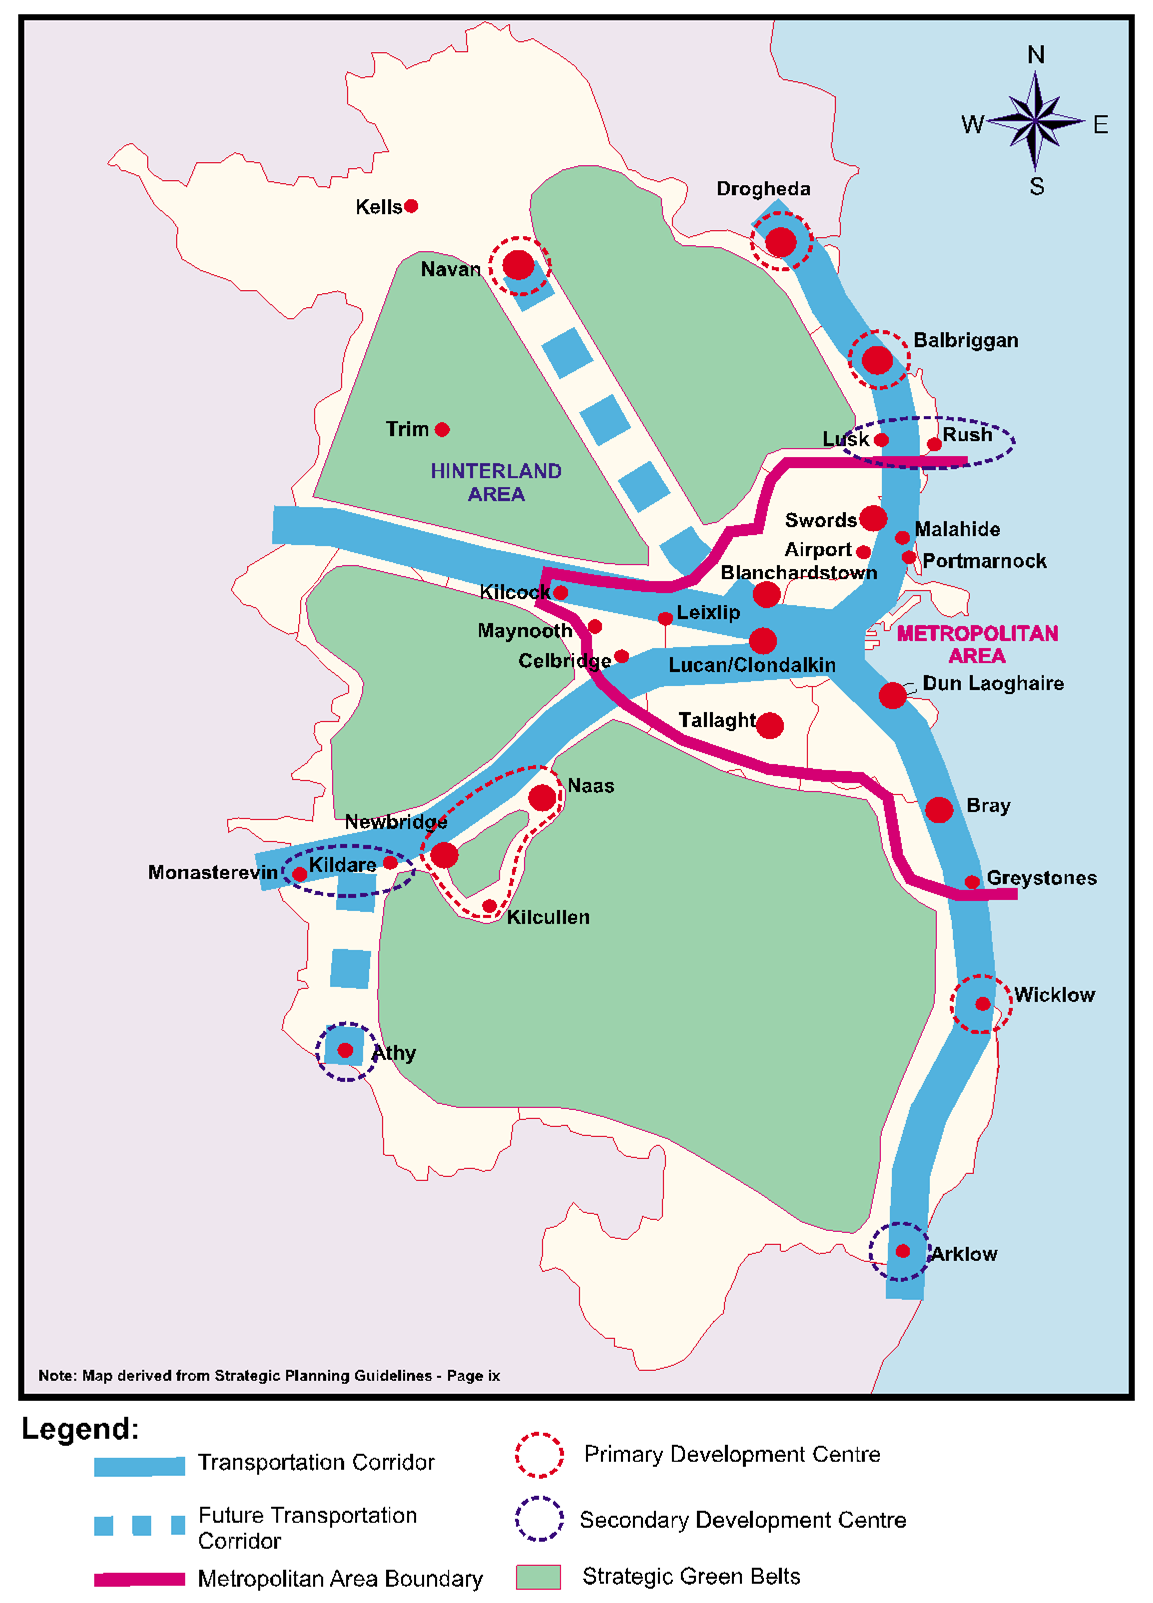
\includegraphics[width=400pt]{intro1}\\
\caption{Map of the Greater Dublin Area \citep{PLA01}} \label{Figure: Map of the Greater Dublin
Area}
\end{figure}
\newpage

\begin{table}[htbp]
\footnotesize{} \setlinespacing{1.0} \vspace{10pt} \begin{longtable} {p{190pt}cccc}
\caption{Demographic Projections of the GDA} \\
\hline

\textbf{Greater Dublin Area}&

\textbf{1991}  & \textbf{1996}& \textbf{1999}& \textbf{2016} \\* \hline \hline {Population
(million) }&

{1.35}  & {1.41}& {1.46}& {1.75} \\* \hline {Households ('000) }&

{402}  & {446}& {521}& {675} \\* \hline {Employment ('000) }&

{452}  & {549}& {681}& {878} \\* \hline {Unemployment rate }&

{16{\%}}  & {12{\%}}& {6{\%}}& {5{\%}} \\* \hline {Car Ownership (per 1000 population)}&

{247}  & {292}& {342}& {480} \\* \hline {{\%} Growth in GDP since 1991}& {- }& {42{\%}}& {79{\%}}&
{260{\%} }\\* \hline

\label{Table: Demographic Projections of the GDA}
\end{longtable}
 \normalsize{} \setlinespacing{1.1}
\end{table}

\newpage

\begin{figure}[htbp]
\center 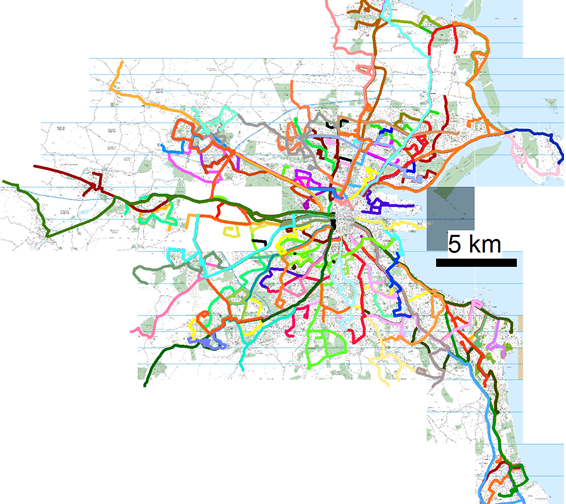
\includegraphics[width=400pt]{intro2}\\
\caption{Map of Bus Routes of Dublin Bus} \label{fig2: Map of bus routes provided by Dublin Bus}
\end{figure}

The figures shown in Table \ref{Table: Demographic Projections of the GDA} are taken from the
website of Dublin Bus \citep{DUB05}. The bus fleet is broken down into depot location and bus
category.

\subsection{Subsection header 2}
fdsdfsdfds
\subsection{Subsection header 3}
fdsdfsdfds
\end{comment}

\section{Justification / Benefits}

\begin{comment}
\subsection{Subsection header 1}
fdsdfsdfds
\subsection{Subsection header 2}
fdsdfsdfds
\subsection{Subsection header 3}
fdsdfsdfds
\end{comment}

When it comes to that time of year where lecturers need to set aside the time to create their examination papers for the modules which they deliver. This is where this project will come into its own with the aim of taking the stress out of the procedure and to provide examiners an easy to use means of examination paper compilation. This usability will come from a combination of a clean and simple user interface along with useful tools to create examination papers.

\section{Feasibility}

\begin{comment}
\subsection{Subsection header 1}

Latex is very good when mathematical formulas need to be displayed:

\begin{equation}\label{taeq2}
    S_{ij}=1-{\frac{|(F_{ij}-F^T_{ij})|}{(F_{ij}+F^T_{ij})}}
\end{equation}


\subsection{Subsection header 2}
\subsection{Subsection header 3}
\end{comment}

Since there are numerous examples of this implementation on the internet. This comes from reading research papers from other students in colleges and technical institutions all around the world. Furthermore the prerequisites obtained from this projects supervisor ensures that the project is technically feasible. However, some research needs to be undertaken regarding the security and encryption aspects. This will be the main technical difficulty and therefore there needs to be a sufficient technical understanding of the technologies involved in order to complete the project.

\section{Proposed Methodologies}

\begin{comment}
\subsection{Subsection header 1}
fdsdfsdfds
\subsection{Subsection header 2}
fdsdfsdfds
\subsection{Subsection header 3}
fdsdfsdfds
\end{comment}

To articulate the methods and techniques used in this plan. Below is the outcome after reviewing various SDLC methodologies with reference to \cite{TP-16}:
\begin{itemize}
	\item Adoption of the Agile Model.
	\item Suits the requirements for this project.
	\item Widely accepted within companies within the IT industry.
	\item Valuable learning curve in gaining experience with this model.
	\item Model has the ability to adapt and tailor itself within each increment as the project moves forward.
	\item Advantageous to the project.
	
\begin{comment}
	\begin{itemize}
		\item A bullet within a bullet!
			\begin{itemize}
				\item Must go deeper...
			\end{itemize}
		\item [Title] Second one too.
	\end{itemize}
	\item Good Things come in threes.
		\item [Title] blah blah blah
		\item [This is a longer title] blah blah blah blah!
			\begin{enumerate}
				\item Some people
				\item Like lists with numbers instead.
			\end{enumerate}
\end{comment}		
\end{itemize}

\begin{comment}
After reviewing the available SDLC methodologies. It has been decided to adopt the Agile Model. Since this best suits the requirements for this project. Adding to this is that it is well recognised as being best practice with companies working within the same field. It would also be a good learning curve in which to gain experience with this model. It can be advantageous to the project as this methodology has the ability to adapt and to tailor itself to each increment of the project as it moves forward.
\end{comment}

\begin{figure}[htbp]
\center 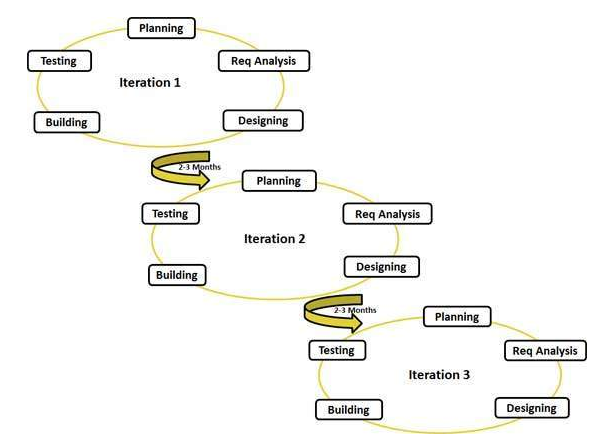
\includegraphics[width=400pt]{Figures/sdlc_agile_model}\\
\caption{Graphical illustration of the Agile Model \citep{TP-16}} \label{Figure: Graphical illustration of the Agile Model}
\end{figure}

\begin{comment}
The diagram shown above \ref{Table: Demographic Projections of the GDA} are taken from the
website of Dublin Bus \citep{TP-16}. The bus fleet is broken down into depot location and bus
category.
\end{comment}

\section{Expected Results}

\begin{comment}
\subsection{Subsection header 1}
fdsdfsdfds
\subsection{Subsection header 2}
fdsdfsdfds
\subsection{Subsection header 3}
fdsdfsdfds
\end{comment}

As noted in the Feasibility section the project should be feasible from a technical standpoint.  It is therefore expected that the project will result in a fully-functioning web site that makes use of the technologies provided.

\section{Conclusion}

\begin{comment}
\subsection{Subsection header 1}
fdsdfsdfds
\subsection{Subsection header 2}
fdsdfsdfds
\subsection{Subsection header 3}
fdsdfsdfds
\end{comment}

This project aims to provide a simple and easy to use service through the use of various Internet technologies combined with automatic generation of question papers and functions. It is hoped that such a service can reduce both the time and difficulties experienced by examiners during an busy time of the year.

\section{Project plan}

\begin{comment}
\subsection{Subsection header 1}
fdsdfsdfds
\subsection{Subsection header 2}
fdsdfsdfds
\subsection{Subsection header 3}
fdsdfsdfds
\end{comment}

Table \ref{table:1} Which shows the Work Breakdown Structure.
 
\begin{table}[h!]
\centering
\begin{tabular}{||c c c c||} 
 \hline
 Task Name & Start & Finish & Duration \\ [0.5ex] 
 \hline\hline
Planning 				& 12/09/16 & 17/10/16 & 42d \\ 
Project Plan 			& 12/09/16 & 26/09/16 & 14d \\
Research Project Ideas	& 12/09/16 & 26/09/16 & 5d \\
Project Proposal 		& 27/09/16 & 12/10/16 & 5d \\
Feasibility Study		& 12/10/16 & 14/10/16 & 13d \\
Research Methodologies 	& 14/09/16 & 16/10/16 & 7d \\
Create Project Proposal   	& 16/10/16 & 26/10/16 & 5d \\
Submit Project Proposal   	& 26/10/16 & 26/10/16 & 0d \\
Literature Review              	& 26/10/16 & 31/10/2016 & 2d \\
Submit Literature Review  & 31/10/2016 & 07/11/2016 & 0d \\
Development                     & 07/11/2016 & 12/12/2016 & 108d \\
Version 1                           	& 12/12/2016 & 12/09/16 & 28d \\
Analysis                            	& 14/09/2016 & 30/09/2016 & 7d \\
User Registration 		& 14/09/2016 & 30/09/2016 & 7d \\
Question Entry 			& 28/10/2016 & 12/09/16 & 7d \\
Create Question Section   & 28/10/2016 & 12/09/16 & 7d \\
Design 				& 28/10/2016 & 31/10/2016 & 7d \\
Use Cases 			& 28/10/2016 & 31/10/2016 & 2d \\
Class Diagrams 		& 31/10/2016 & 07/11/2016 & 2d \\
ERDs 				& 31/10/2016 & 07/11/2016 & 2d \\
Wireframes 			& 31/10/2016 & 07/11/2016 & 1d \\
Implementation 		& 31/10/2016 & 12/09/16 & 14d \\
Database Creation 		& 31/10/2016 & 07/11/2016 & 2d \\
Home Page 			& 31/10/2016 & 07/11/2016 & 3d \\
User Registration 		& 31/10/2016 & 07/11/2016 & 4d \\
Question Entry Page 	& 31/10/2016 & 07/11/2016 & 4d \\
Deliver Version 1 		& 07/11/2016 & 12/12/2016 & 0d \\
Testing 				& 07/11/2016 & 12/12/2016 & 11d \\
Review Version 1 		& 07/11/2016 & 12/12/2016 & 7d \\
Analysis 				& 07/11/2016 & 12/12/2016 & 7d \\
View Listings 			& 07/11/2016 & 12/12/2016 & 7d \\
Show Questions 		& 12/12/2016 & 12/12/2016 & 7d \\
Generate Questions 		& 12/12/2016 & 15/12/2016 & 7d \\
Design 				& 12/12/2016& 15/12/2016 & 7d \\
Use Cases 			& 12/12/2016 & 15/12/2016 & 3d \\
Wireframes 			& 12/12/2016 & 15/12/2016 & 2d \\
ERDs 				& 12/12/2016 & 15/12/2016 & 3d \\
Implementation 		& 09/01/2017 & 15/12/2016 & 14d \\
Database Changes 		& 09/01/2017 & 15/12/2016 & 2d \\
View Questions Page 	& 09/01/2017 & 09/01/2017 & 4d \\
Generate Question Page 	& 09/01/2017 & 09/01/2017 & 4d \\
Testing 				& 09/01/2017 & 09/01/2017 & 12 \\
Deliver Version 2 		& 09/01/2017 & 09/01/2017 & 7d \\
												
 \hline
\end{tabular}
\caption{Table to represent the Work Breakdown Structure}
\label{table:1}
\end{table}

\begin{figure}[htbp]
\center 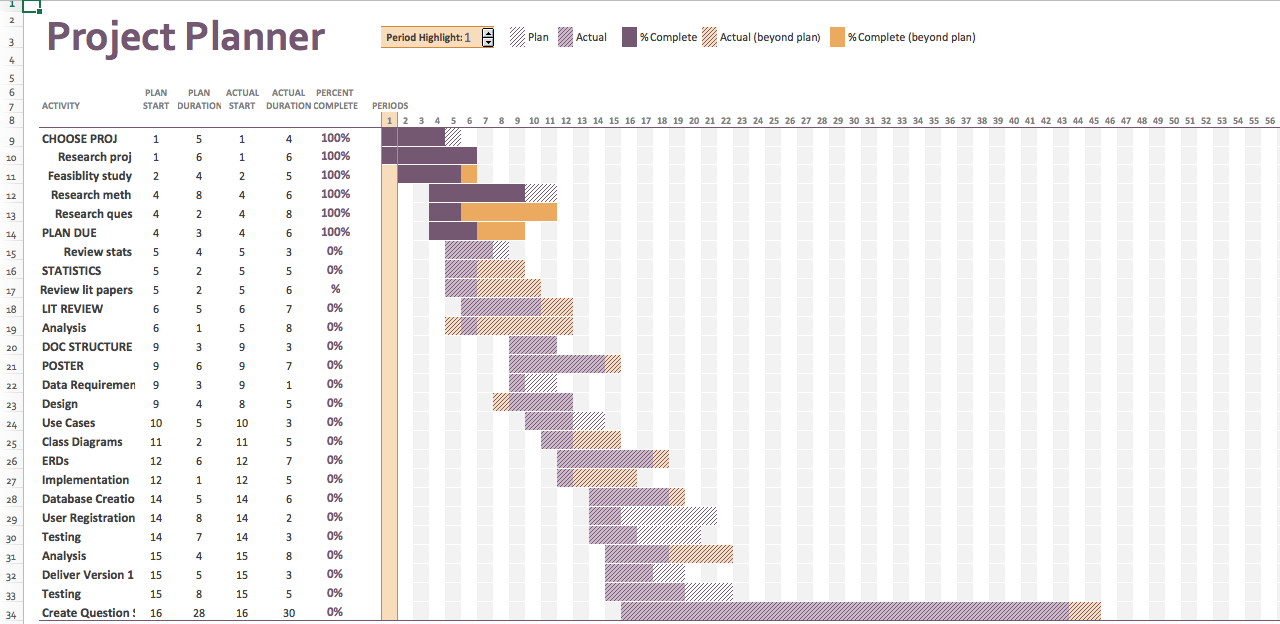
\includegraphics[width=400pt]{Figures/gantt}\\
\caption{Gantt Chart} \label{Figure: Gantt Chart}
\end{figure}
